\let\negmedspace\undefined
\let\negthickspace\undefined
\documentclass[journal]{IEEEtran}
\usepackage[a5paper, margin=10mm, onecolumn]{geometry}
%\usepackage{lmodern} % Ensure lmodern is loaded for pdflatex
\usepackage{tfrupee} % Include tfrupee package

\setlength{\headheight}{1cm} % Set the height of the header box
\setlength{\headsep}{0mm}     % Set the distance between the header box and the top of the text

\usepackage{gvv-book}
\usepackage{gvv}
\usepackage{cite}
\usepackage{amsmath,amssymb,amsfonts,amsthm}
\usepackage{algorithmic}
\usepackage{graphicx}
\usepackage{textcomp}
\usepackage{xcolor}
\usepackage{txfonts}
\usepackage{listings}
\usepackage{enumitem}
\usepackage{mathtools}
\usepackage{gensymb}
\usepackage{comment}
\usepackage[breaklinks=true]{hyperref}
\usepackage{tkz-euclide} 
\usepackage{listings}
% \usepackage{gvv}                                        
\def\inputGnumericTable{}                                 
\usepackage[latin1]{inputenc}                                
\usepackage{color}                                            
\usepackage{array}                                            
\usepackage{longtable}                                       
\usepackage{calc}                                             
\usepackage{multirow}                                         
\usepackage{hhline}                                           
\usepackage{ifthen}                                           
\usepackage{lscape}
\begin{document}

\bibliographystyle{IEEEtran}
\vspace{3cm}
\title{11.16.2.2.6}
\author{EE24BTECH11025 - GEEDI HARSHA}
% \maketitle
% \newpage
{\let\newpage\relax\maketitle}

\renewcommand{\thefigure}{\theenumi}
\renewcommand{\thetable}{\theenumi}
\setlength{\intextsep}{10pt} % Space between text and floats


\numberwithin{equation}{enumi}
\numberwithin{figure}{enumi}
\renewcommand{\thetable}{\theenumi}







\textbf{Question:} A die is thrown. Describe the following event:  

(a) \( F \): a number not less than 3.

\textbf{Solution:}

A fair six-sided die has outcomes in the sample space:

\begin{align}
    S &= \{1, 2, 3, 4, 5, 6\}.
\end{align}

The event \( F \) represents getting a number not less than 3, which means:

\begin{align}
    F &= \{3, 4, 5, 6\}.
\end{align}

Since the die is fair, each face has an equal probability of occurring. The probability mass function (PMF) describes the probability of each outcome:

\begin{align}
    P(X = x) &= \frac{1}{6}, \quad x \in \{1, 2, 3, 4, 5, 6\}.
\end{align}

The cumulative distribution function (CDF) gives the probability of rolling a number less than or equal to \( x \):

\begin{align}
    P(X \leq x) &= \sum_{k=1}^{x} P(X = k) = \frac{x}{6}, \quad x \in \{1, 2, 3, 4, 5, 6\}.
\end{align}

The probability of event \( F \) occurring is calculated as follows:

\begin{align}
    P(F) &= \frac{\text{Number of favorable outcomes}}{\text{Total number of outcomes}}. \\
         &= \frac{4}{6} = \frac{2}{3}.
\end{align}

Thus, the probability of rolling a number not less than 3 is \( \frac{2}{3} \).

This means that in a large number of trials, about \( 66.67\% \) of the rolls will yield a number between 3 and 6.
\begin{figure}[h]
    \centering
    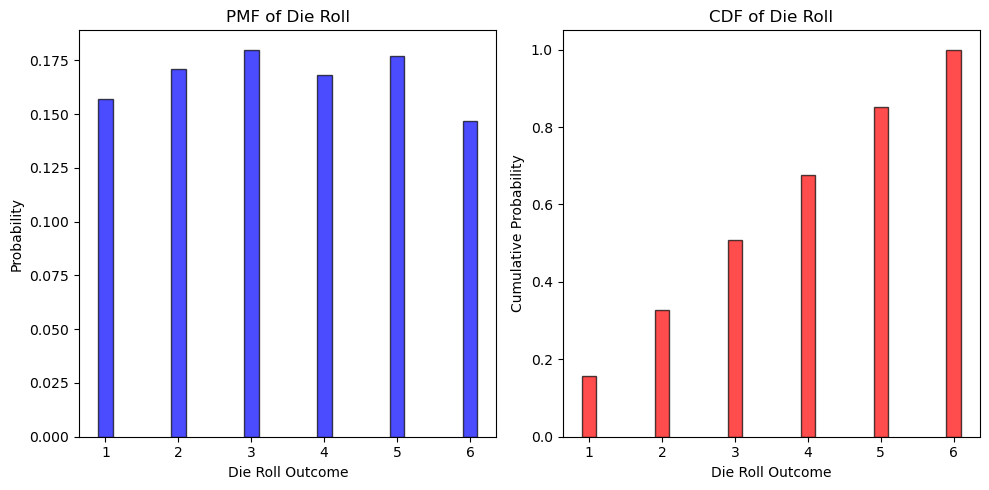
\includegraphics[width=\textwidth]{figs/fig.png}
\end{figure}
\end{document}

